% File for libamtrack manual
% Copyright 2006, 2010 Steffen Greilich / the libamtrack team
% This file is part of the libAmTrack project (libamtrack.dkfz.org).

\chapter{Photon response models}
\label{chap:GRs}

For the actual computation of HCP response, several photon-response relations are found in libamtrack (Tab. \ref{tbl:GRs} and and Fig. \ref{fig:GRs}). Again, they can almost freely combined with the ATMs (an important exception still being IGK which is bound to a general hit/target response).


\begin{table}
\label{tbl:table4}
\begin{tabular}{m{0.25\textwidth}p{0.60\textwidth}m{0.15\textwidth}}

\hline
\textbf{Name} & \textbf{Expression} & \textbf{Reference} \\
\hline

\begin{center}Test\end{center}&
$S(D)=a\cdot D+b$&
\textsl{simple linear function}\\

\begin{center}General hit/target\end{center}&
$S(D)=(1-sum_{k=0}^{c-1}{\frac{(D/D_0)^k}{k!}\cdot e^{-(D/D_0)}})^m$
&\cite{Dertinger_and_Jung_1970}\\

\begin{center}Radioluminescence\end{center}&
$S(D)=\begin{cases}c_1\cdot D+c_2 \cdot D^2&\text{if $D<D_{sat}$,}\\
c_3+c_4 \cdot D&\text{if $D\ge D_{sat}$,}
\end{cases}$&\cite{Andersen_et_al_2006}, \cite{Greilich_et_al_2008}\\

\begin{center}Exp.-saturation\end{center}&
$S(D)=c\cdot (1-e^{-D/D_0})$
&\textsl{simplified case of the general hit/target model}\\

\begin{center}Linear-quadratic\end{center}&
$S(D)=e^{-\alpha\cdot D-\beta \cdot D^2}$
&\cite{Chadwick_and_Leenhouts_1973}\\

\hline
\end{tabular}
\caption{Photons response models implemented in \la{}.}
\end{table}


\begin{figure*}
	\centering
		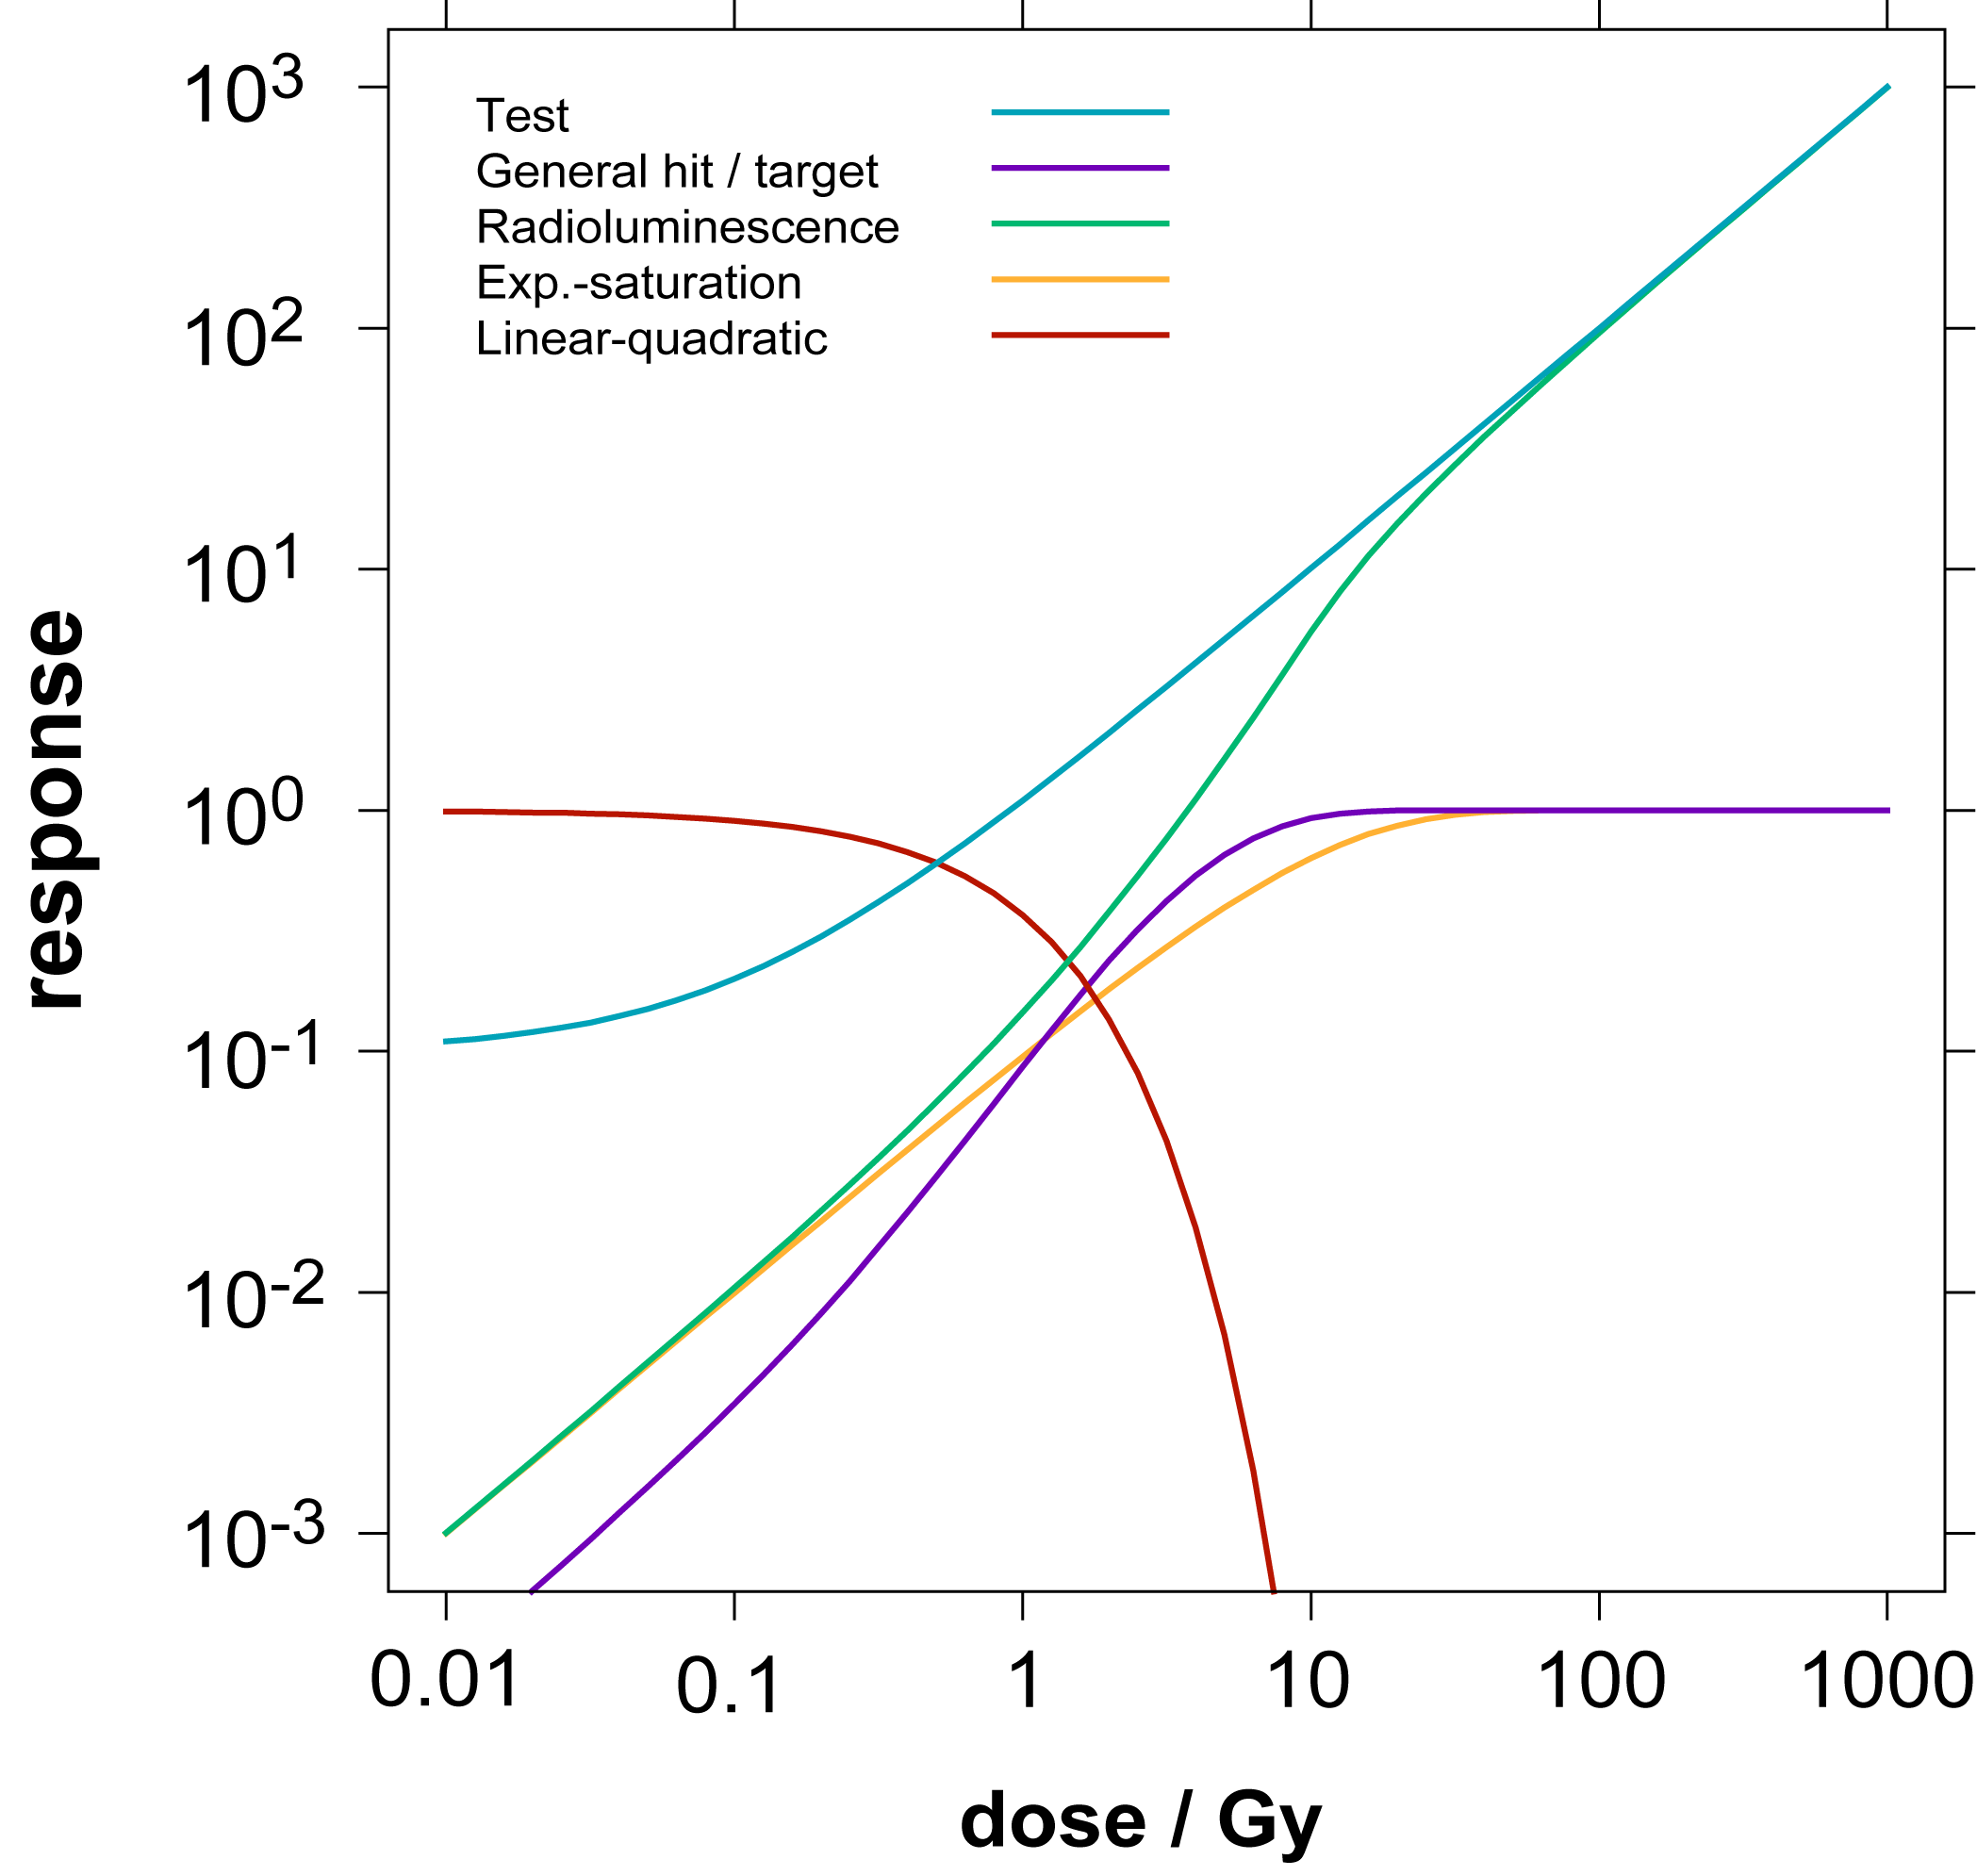
\includegraphics[bb=0 0 2097 1990,width=1.0\textwidth]{pictures/GR.png}
	\caption{Photon-responses available in \la{}.}
	\label{fig:GRs}
\end{figure*}


\section*{Document status}
\begin{tabular}{l l}
2010.06.01&Created by S. Greilich
\end{tabular}